\titledquestion{Trees}

Each question has \textbf{one or more than one} correct answer(s). Please answer the following questions \textbf{according to  the definition specified in the lecture slides}.

%%%%%%%%%%%%%%%%%%%%%%%%%%%%%%%%%%%%%%%%%%%%%%%%%%%%%%%%%%%%%%%%%%%%%%%%%%%
% Note: The `LaTeX' way to answer a multiple-choices question is to replace `\choice'
% with `\CorrectChoice', as what you did in the previous questions. However, there are 
% still many students who would like to handwrite their homework. To make TA's work 
% easier, you have to fill your selected choices in the table below, no matter whether 
% you use LaTeX or not.
%%%%%%%%%%%%%%%%%%%%%%%%%%%%%%%%%%%%%%%%%%%%%%%%%%%%%%%%%%%%%%%%%%%%%%%%%%%

\begin{table}[htbp]
	\centering
	\begin{tabular}{|p{2cm}|p{2cm}|p{2cm}|}
		\hline
		(a) & (b) & (c) \\
		\hline
		%%%%%%%%%%%%%%%%%%%%%%%%%%%%%%%%%%%%%%%%%%%%%%%%%%%%%%%%%%
		% YOUR ANSWER HERE.
		 ABD   &  A   &  A   \\
		%%%%%%%%%%%%%%%%%%%%%%%%%%%%%%%%%%%%%%%%%%%%%%%%%%%%%%%%%%
		\hline
	\end{tabular}
\end{table}

\begin{parts}
	\part[3] Which of the following statements is(are) \textbf{false}?

	\begin{choices}
        \CorrectChoice Nodes with the same depth are siblings.
        \CorrectChoice Each node in a tree has exactly one parent pointing to it.
        \choice Given any node $a$ within a tree, the collection of $a$ and all of its descendants is a subtree of the tree with root $a$.
        \CorrectChoice The root node cannot be the descendant of any node.
        \choice Nodes with degree zero are called leaf nodes.
        \choice Any tree can be converted into a forest by removing the root node.
	\end{choices}

	\part[3] {Given the following pseudo-code, what kind of traversal does it implement?}

    \begin{center}
    \begin{minipage}{.7\linewidth}
        \begin{algorithm}[H]
            \begin{algorithmic}[1]
                \Function {order}{node}			
                \State visit(node)
        
                \If{node has left child}
                \State order(node.left)
                \EndIf
        
                \If{node has right child}
                \State order(node.right)
                \EndIf 
        
                \EndFunction
            \end{algorithmic}
        \end{algorithm}
    \end{minipage}
    \end{center}

	\begin{choices}
        \CorrectChoice Preorder depth-first traversal
        \choice Postorder depth-first traversal
        \choice Inorder depth-first traversal
        \choice Breadth-first traversal
	\end{choices}

    \newpage

	\part[3] Which traversal strategy should we use if we want to print the hierarchical structure?

    \begin{figure}[h]
        \centering
        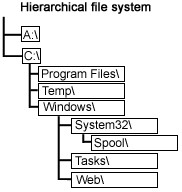
\includegraphics[width=0.27\linewidth]{hierarchy}
    \end{figure}
		
	\begin{choices}
        \CorrectChoice CorrectChoice depth-first traversal
        \choice Postorder depth-first traversal
        \choice Inorder depth-first traversal
        \choice Breadth-first traversal
	\end{choices}
\end{parts}